% 'draft' mode can be used to speed up compilation
\documentclass[twoside,final]{hcmut-report}

% Times New Roman font
\usepackage{mathptmx}

% Encodings
\usepackage{gensymb,textcomp}

% Better tables
\usepackage{array,longtable,multicol,multirow,siunitx,tabularx}

% Better enum
\usepackage{enumitem}

% Graphics
\usepackage{caption,float}

% Add options for figures, like max width, framing, etc.
\usepackage[export]{adjustbox}

% References
\usepackage[nameinlink]{cleveref}

% Configurations
\coursename{HÓA ĐẠI CƯƠNG (TN) (CH1004)}
\reporttype{BÀI BÁO CÁO THÍ NGHIỆM HÓA ĐẠI CƯƠNG}
\title{BẢN BÁO CÁO SỐ LIỆU THÍ NGHIỆM\\[1cm]\large{Nhóm báo cáo: Nhóm 2 - Lớp L55 - Học kỳ 252}}
\advisor{& Nguyễn Thị Thanh Phượng &}
\stuname{%
  & Hồ Anh Dũng & 2310543 \\
  & Phạm Gia Huy & 2411256 \\
}

\reportplace{Thành phố Hồ Chí Minh}
\reporttime{tháng 04 năm 2026}

% Set depth of numbering for counters
\AtBeginDocument{\counterwithin{table}{section}}

% Rename some sections
\AtBeginDocument{\renewcommand*{\contentsname}{MỤC LỤC}}
\AtBeginDocument{\renewcommand*{\listfigurename}{DANH MỤC HÌNH ẢNH}}
\AtBeginDocument{\renewcommand*{\listtablename}{DANH MỤC BẢNG BIỂU}}

\begin{document}
\coverpage%

\tableofcontents
\listoffigures
\listoftables
%\lstlistoflistings{}

\clearpage

\section{BÀI 2. NHIỆT PHẢN ỨNG}
\subsection{THÍ NGHIỆM}
\subsubsection{Thí nghiệm 1: Xác định nhiệt dung của nhiệt lượng kế}
\textbf{a. Tiến trình thí nghiệm}
\begin{itemize}
    \item Dùng ống đong lấy 50ml nước nguội cho vào becher rồi để thẳng nhiệt kế đo nhiệt độ $t_1$.
    \item Dùng ống đong lấy 50ml nước sôi (60-70$^\circ$C) cho vào nhiệt lượng kế rồi đo nhiệt độ $t_2$.
    \item Dùng phễu cho nhanh 50ml nước nguội vào nhiệt lượng kế rồi lắc đều cho nhiệt độ ổn định ta đo nhiệt độ $t_3$.
    \item Sử dụng công thức: $m_0c_0 = \frac{mc(t_3 - t_1) - (t_2 - t_3)}{t_2 - t_3}$
    \item Chú ý:
    \begin{itemize}
        \item m = khối lượng 50ml nước
        \item c = 1 cal/g.độ
        \item $0 < m_0c_0 < 12$
    \end{itemize}
\end{itemize}

\textbf{b. Kết quả}
\begin{itemize}
    \item Bảng số liệu:
    \begin{table}[H]
        \centering
        \begin{tabular}{|c|c|c|c|}
            \hline
            & \textbf{Lần 1} & \textbf{Lần 2} & \textbf{Lần 3} \\
            \hline
            $t_1$ & 29 & & \\
            \hline
            $t_2$ & 66 & & \\
            \hline
            $t_3$ & 48 & & \\
            \hline
            $m_0c_0$ & 2.78 & & \\
            \hline
        \end{tabular}
    \end{table}
    \item Tính giá trị $m_0c_0$:
    $$m_0c_0 = \frac{mc(t_3 - t_1) - (t_2 - t_3)}{t_2 - t_3} = \frac{50 \cdot (48 - 29) - (66 - 48)}{66 - 48} = 2.78 \text{ (cal/độ)}$$
\end{itemize}

\subsubsection{Thí nghiệm 2: Xác định hiệu ứng nhiệt của phản ứng trung hòa dung dịch HCl và NaOH}
\textbf{a. Tiến trình thí nghiệm}
\begin{itemize}
    \item Tráng buret 25ml bằng dung dịch NaOH 1M rồi lấy 25ml dung dịch NaOH 1M cho vào becher, đo nhiệt độ $t_1$.
    \item Tráng buret 25ml bằng dung dịch HCl 1M rồi lấy 25ml dung dịch HCl 1M cho vào nhiệt lượng kế, đo nhiệt độ $t_2$.
    \item Dùng phễu cho 25ml dung dịch NaOH vào nhiệt lượng kế, đo nhiệt độ $t_3$.
    \item Sử dụng công thức: $Q = (m_0c_0 + mc)(t_3 - \frac{t_1 + t_2}{2}) \text{ (cal)}$
    \item Chú ý:
    \begin{itemize}
        \item $m_{dd} = dV_{dd} \text{ (d = 1.02 g/ml)}$
        \item $c_{dd} = 1 \text{ cal/g.độ}$
        \item $\Delta H = -\frac{Q}{n}$
    \end{itemize}
\end{itemize}

\textbf{b. Kết quả}
\begin{itemize}
    \item Bảng số liệu:
    \begin{table}[H]
        \centering
        \begin{tabular}{|c|c|c|c|}
            \hline
            & \textbf{Lần 1} & \textbf{Lần 2} & \textbf{Lần 3} \\
            \hline
            $t_1$ & 29.5 & 29.5 & \\
            \hline
            $t_2$ & 30.1 & 30.5 & \\
            \hline
            $t_3$ & 35 & 35 & \\
            \hline
            $Q$ & 279.656 & 268.9 & \\
            \hline
            $Q$ trung bình & \multicolumn{3}{c|}{274.278} \\
            \hline
            $\Delta H$ & -11186.24 & -10756 & \\
            \hline
            $\Delta H$ trung bình & \multicolumn{3}{c|}{-10971.12} \\
            \hline
        \end{tabular}
    \end{table}
    \item Tính giá trị Q và $\Delta H$:
    \begin{align*}
        V_{dd} &= 25 + 25 = 50 \text{ (ml)} \\
        m &= d \times V_{dd} = 50 \times 1.02 = 51 \text{ (g)} \\
        m_0c_0 &= 2.78 \\
        Q &= (m_0c_0 + mc)\left(t_3 - \frac{t_1 + t_2}{2}\right) \\
          &= (2.78 + 51 \times 1)\left(35 - \frac{29.5 + 30.1}{2}\right) = 279.656 \text{ (cal)}
    \end{align*}
    Phương trình hóa học:
    \begin{align*}
        &\text{NaOH} + \text{HCl} \rightarrow \text{NaCl} + \text{H}_2\text{O} \\
        &0.025 \quad 0.025 \quad 0.025 \\
        \Delta H &= -\frac{Q}{n} = -\frac{279.656}{0.025} = -11186.24 \text{ (cal/mol)}
    \end{align*}
    \item Kết luận: Vì $\Delta H < 0$ nên đây là phản ứng tỏa nhiệt.
\end{itemize}

\subsubsection{Thí nghiệm 3: Xác định nhiệt hòa tan của CuSO\textsubscript{4} khan}
\textbf{a. Tiến trình thí nghiệm}
\begin{itemize}
    \item Dùng ống đong lấy 50ml nước vào nhiệt lượng kế rồi đo nhiệt độ $t_1$.
    \item Cân 4g CuSO\textsubscript{4} khan rồi cho vào nhiệt lượng kế rồi đo nhiệt độ $t_2$.
    \item Sử dụng công thức: $Q = (m_0c_0 + mc)(t_2 - t_1) \text{ (cal)}$
    \item Chú ý:
    \begin{itemize}
        \item $m_{dd} = m_{ct} + m_{dm}$
        \item $c_{dd} = 1 \text{ cal/g.độ}$
        \item $\Delta H = -\frac{Q}{n}$
    \end{itemize}
\end{itemize}

\textbf{b. Kết quả}
\begin{itemize}
    \item Bảng số liệu:
    \begin{table}[H]
        \centering
        \begin{tabular}{|c|c|c|c|}
            \hline
            & \textbf{Lần 1} & \textbf{Lần 2} & \textbf{Lần 3} \\
            \hline
            $t_1$ & 30 & 30 & \\
            \hline
            $t_2$ & 35.5 & 35 & \\
            \hline
            m (cân) & 3.7 & 3.85 & \\
            \hline
            $\Delta t$ & 5.5 & 5 & \\
            \hline
            $Q$ & 310.64 & 283.15 & \\
            \hline
            $\Delta H$ & -13433.081 & -11767.273 & \\
            \hline
            $\Delta H$ trung bình & \multicolumn{3}{c|}{-12600.177} \\
            \hline
        \end{tabular}
    \end{table}
    \item Tính giá trị Q và $\Delta H$:
    \begin{align*}
        m_{dd} &= m_{ct} + m_{dm} = 3.7 + 50 = 53.7 \\
        n_{CuSO_4} &= \frac{3.7}{160} = 0.023125 \text{ (mol)} \\
        Q &= (m_0c_0 + mc)\Delta t \\
          &= (2.78 + 53.7 \times 1) \times 5.5 = 310.64 \text{ (cal)} \\
        \Delta H &= -\frac{Q}{n} = -\frac{310.64}{0.023125} = -13433.081 \text{ (cal/mol)}
    \end{align*}
    \item Kết luận: Vì $\Delta H < 0$ nên đây là phản ứng tỏa nhiệt.
\end{itemize}

\subsubsection{Thí nghiệm 4: Xác định nhiệt hòa tan NH\textsubscript{4}Cl khan}
\textbf{a. Tiến trình thí nghiệm}
\begin{itemize}
    \item Tương tự thí nghiệm 3 nhưng thay CuSO\textsubscript{4} khan bằng NH\textsubscript{4}Cl khan.
    \item Sử dụng công thức tương tự thí nghiệm 3.
\end{itemize}

\textbf{b. Kết quả}
\begin{itemize}
    \item Bảng số liệu:
    \begin{table}[H]
        \centering
        \begin{tabular}{|c|c|c|c|}
            \hline
            & \textbf{Lần 1} & \textbf{Lần 2} & \textbf{Lần 3} \\
            \hline
            $t_1$ & 30 & 30 & \\
            \hline
            $t_2$ & 27 & 26 & \\
            \hline
            m (cân) & 3.55 & 3.59 & \\
            \hline
            $\Delta t$ & -3 & -4 & \\
            \hline
            $Q$ & -168.99 & -225.48 & \\
            \hline
            $\Delta H$ & 2546.75 & 3360.217 & \\
            \hline
            $\Delta H$ trung bình & \multicolumn{3}{c|}{2953.484} \\
            \hline
        \end{tabular}
    \end{table}
    \item Tính giá trị Q và $\Delta H$:
    \begin{align*}
        m_{dd} &= m_{ct} + m_{dm} = 3.55 + 50 = 53.55 \\
        n_{NH_4Cl} &= \frac{3.55}{53.5} = 0.066 \text{ (mol)} \\
        Q &= (m_0c_0 + mc)\Delta t \\
          &= (2.78 + 53.55 \times 1) \times -3 = -168.99 \text{ (cal)} \\
        \Delta H &= -\frac{Q}{n} = -\frac{-168.99}{0.066} = 2546.75 \text{ (cal/mol)}
    \end{align*}
    \item Kết luận: Vì $\Delta H > 0$ nên đây là phản ứng thu nhiệt.
\end{itemize}

\subsection{TRẢ LỜI CÂU HỎI}
\begin{enumerate}
    \item \textbf{$\Delta H_{tb}$ của phản ứng HCl + NaOH $\rightarrow$ NaCl + H\textsubscript{2}O sẽ được tính theo số mol HCl hay NaOH khi cho 25 ml dd HCl 2M tác dụng với 25 ml dd NaOH 1M. Tại sao?}
    \begin{itemize}
        \item $n_{HCl} = 0.025 \times 2 = 0.05 \text{ (mol)}$
        \item $n_{NaOH} = 0.025 \times 1 = 0.025 \text{ (mol)}$
        \item Ta thấy $n_{HCl} > n_{NaOH}$ nên NaOH phản ứng hết còn HCl thì còn dư $\rightarrow \Delta H_{tb}$ phản ứng được tính dựa trên số mol chất phản ứng nên sẽ được tính theo số mol NaOH.
    \end{itemize}
    \item \textbf{Nếu thay HCl 1M bằng HNO\textsubscript{3} 1M thì kết quả thí nghiệm 2 có thay đổi hay không?}
    Kết quả thí nghiệm 2 không thay đổi vì HNO\textsubscript{3} cũng là một axit mạnh, phân li hoàn toàn và tác dụng với NaOH cũng là một phản ứng trung hòa.
    \item \textbf{Tính $\Delta H_3$ bằng lý thuyết theo định luật Hess. So sánh với kết quả thí nghiệm. Hãy xem 6 nguyên nhân có thể gây ra sai số trong thí nghiệm này?}
    \begin{itemize}
        \item Mất nhiệt độ do nhiệt lượng kế.
        \item Do nhiệt kế.
        \item Do dụng cụ đong thể tích hóa chất.
        \item Do cân.
        \item Do sunfat đồng bị hút ẩm.
        \item Do lấy nhiệt dung riêng của dung dịch sunfat đồng bằng 1 cal/mol.độ.
    \end{itemize}
    \textbf{Theo em sai số nào là quan trọng nhất, giải thích? Còn nguyên nhân nào khác không?}
    \begin{itemize}
        \item Theo định luật Hess: $\Delta H_3 = \Delta H_1 + \Delta H_2 = -18.7 + 2.8 = -15.9 \text{ (kcal/mol)}$
        \item Theo thực nghiệm: $\Delta H_3 = -14.5488 \text{ (kcal/mol)}$
        \item $\rightarrow$ Chênh lệch quá lớn
        \item Theo em nguyên nhân gây ra sai số có thể là:
        \begin{itemize}
            \item Mất nhiệt độ do nhiệt lượng kế do trong quá trình thí nghiệm thao tác không chính xác, nhanh chóng dẫn đến thoát nhiệt ra môi trường bên ngoài.
            \item Sunfat đồng bị hút ẩm do trong lúc cân và đưa vào thí nghiệm thao tác không nhanh chóng.
        \end{itemize}
    \end{itemize}
\end{enumerate}

\section{BÀI 4. XÁC ĐỊNH BẬC PHẢN ỨNG}
\subsection{THÍ NGHIỆM}
\subsubsection{Thí nghiệm 1: Xác định bậc phản ứng theo Na\textsubscript{2}S\textsubscript{2}O\textsubscript{3}}
\textbf{a. Tiến trình thí nghiệm}
\begin{itemize}
    \item Chuẩn bị 3 ống nghiệm chứa H\textsubscript{2}SO\textsubscript{4} và 3 bình tam giác chứa Na\textsubscript{2}S\textsubscript{2}O\textsubscript{3} và H\textsubscript{2}O theo bảng sau:
    \begin{table}[H]
        \centering
        \begin{tabular}{|c|c|c|c|}
            \hline
            \multirow{2}{*}{\textbf{TN}} & \textbf{Ống nghiệm} & \multicolumn{2}{c|}{\textbf{Erlen}} \\
            \cline{2-4}
            & \textbf{V(ml) H\textsubscript{2}SO\textsubscript{4} 0.4M} & \textbf{V(ml) Na\textsubscript{2}S\textsubscript{2}O\textsubscript{3} 0.1M} & \textbf{V(ml) H\textsubscript{2}O} \\
            \hline
            1 & 8 & 4 & 28 \\
            \hline
            2 & 8 & 8 & 24 \\
            \hline
            3 & 8 & 16 & 16 \\
            \hline
        \end{tabular}
    \end{table}
    \item Dùng Pipet vạch lấy axit cho vào ống nghiệm.
    \item Dùng Buret cho nước vào 3 Erlen.
    \item Tráng Buret bằng Na\textsubscript{2}S\textsubscript{2}O\textsubscript{3} 0.1M rồi tiếp tục dùng Buret cho Na\textsubscript{2}S\textsubscript{2}O\textsubscript{3} vào 3 Erlen.
    \item Lần lượt cho phản ứng từng cặp ống nghiệm và Erlen như sau:
    \begin{itemize}
        \item Đổ nhanh axit trong ống nghiệm vào Erlen.
        \item Bấm đồng hồ (khi 2 dung dịch tiếp xúc nhau).
        \item Lắc nhẹ, sau đó để yên quan sát, khi thấy dung dịch chuyển sang đục thì bấm dừng đồng hồ.
    \end{itemize}
    \item Lặp lại thí nghiệm lấy giá trị trung bình.
\end{itemize}

\textbf{b. Kết quả}
\begin{itemize}
    \item Bảng số liệu:
    \begin{table}[H]
        \centering
        \begin{tabular}{|c|c|c|c|c|c|}
            \hline
            \textbf{TN} & \textbf{[Na\textsubscript{2}S\textsubscript{2}O\textsubscript{3}]} & \textbf{[H\textsubscript{2}SO\textsubscript{4}]} & \textbf{$\Delta t_1$} & \textbf{$\Delta t_2$} & \textbf{$\Delta t_{TB}$} \\
            \hline
            1 & 0.01 & 0.08 & 142.1 & 130 & 136.05 \\
            \hline
            2 & 0.02 & 0.08 & 75.4 & 67.4 & 71.4 \\
            \hline
            3 & 0.04 & 0.08 & 33.2 & 45.6 & 39.4 \\
            \hline
        \end{tabular}
    \end{table}
    \item Ta có: $m = \frac{\log\left(\frac{\Delta t_1}{\Delta t_2}\right)}{\log(2)}$
    \item Từ TN1 và TN2 ta có: $m_1 = \frac{\log\left(\frac{\Delta t_1}{\Delta t_2}\right)}{\log(2)} = \frac{\log\left(\frac{136.05}{71.4}\right)}{\log(2)} \approx 0.93$
    \item Từ TN2 và TN3 ta có: $m_2 = \frac{\log\left(\frac{\Delta t_2}{\Delta t_3}\right)}{\log(2)} = \frac{\log\left(\frac{71.4}{39.4}\right)}{\log(2)} \approx 0.86$
    \item Bậc phản ứng theo Na\textsubscript{2}S\textsubscript{2}O\textsubscript{3}: $m = \frac{m_1 + m_2}{2} = \frac{0.93 + 0.86}{2} = 0.895$
\end{itemize}

\subsubsection{Thí nghiệm 2: Xác định bậc phản ứng theo H\textsubscript{2}SO\textsubscript{4}}
\textbf{a. Tiến trình thí nghiệm}
\begin{itemize}
    \item Thao tác tương tự phần 1 với lượng axit và Na\textsubscript{2}S\textsubscript{2}O\textsubscript{3} theo bảng sau:
    \begin{table}[H]
        \centering
        \begin{tabular}{|c|c|c|c|}
            \hline
            \multirow{2}{*}{\textbf{TN}} & \textbf{Ống nghiệm} & \multicolumn{2}{c|}{\textbf{Erlen}} \\
            \cline{2-4}
            & \textbf{V(ml) H\textsubscript{2}SO\textsubscript{4} 0.4M} & \textbf{V(ml) Na\textsubscript{2}S\textsubscript{2}O\textsubscript{3} 0.1M} & \textbf{V(ml) H\textsubscript{2}O} \\
            \hline
            1 & 4 & 8 & 1 \\
            \hline
            2 & 8 & 8 & 2 \\
            \hline
            3 & 16 & 8 & 3 \\
            \hline
        \end{tabular}
    \end{table}
\end{itemize}

\textbf{b. Kết quả}
\begin{itemize}
    \item Bảng số liệu:
    \begin{table}[H]
        \centering
        \begin{tabular}{|c|c|c|c|c|c|}
            \hline
            \textbf{TN} & \textbf{[Na\textsubscript{2}S\textsubscript{2}O\textsubscript{3}]} & \textbf{[H\textsubscript{2}SO\textsubscript{4}]} & \textbf{$\Delta t_1$} & \textbf{$\Delta t_2$} & \textbf{$\Delta t_{TB}$} \\
            \hline
            1 & 0.02 & 0.04 & 73.6 & 73.4 & 73.5 \\
            \hline
            2 & 0.02 & 0.08 & 70 & 65.9 & 67.95 \\
            \hline
            3 & 0.02 & 0.16 & 56.3 & 58.5 & 57.4 \\
            \hline
        \end{tabular}
    \end{table}
    \item Từ TN1 và TN2 ta có: $n_1 = \frac{\log\left(\frac{\Delta t_1}{\Delta t_2}\right)}{\log(2)} = \frac{\log\left(\frac{73.5}{67.95}\right)}{\log(2)} \approx 0.11$
    \item Từ TN2 và TN3 ta có: $n_2 = \frac{\log\left(\frac{\Delta t_2}{\Delta t_3}\right)}{\log(2)} = \frac{\log\left(\frac{67.95}{57.4}\right)}{\log(2)} \approx 0.24$
    \item Bậc phản ứng theo H\textsubscript{2}SO\textsubscript{4}: $n = \frac{n_1 + n_2}{2} = \frac{0.11 + 0.24}{2} = 0.175$
\end{itemize}

\subsection{TRẢ LỜI CÂU HỎI}
\begin{enumerate}
    \item \textbf{Trong thí nghiệm trên nồng độ [Na\textsubscript{2}S\textsubscript{2}O\textsubscript{3}] và của [H\textsubscript{2}SO\textsubscript{4}] đã ảnh hưởng thế nào lên vận tốc phản ứng. Viết lại biểu thức tính vận tốc phản ứng. Xác định bậc của phản ứng?}
    \begin{itemize}
        \item Nồng độ [Na\textsubscript{2}S\textsubscript{2}O\textsubscript{3}] tỉ lệ thuận với tốc độ phản ứng.
        \item Nồng độ [H\textsubscript{2}SO\textsubscript{4}] hầu như không ảnh hưởng tới tốc độ phản ứng.
        \item Biểu thức tính vận tốc: $V = k \cdot [\text{Na}_2\text{S}_2\text{O}_3]^{0.9} \cdot [\text{H}_2\text{SO}_4]^{0.07}$
        \item Bậc của phản ứng: $0.9 + 0.07 = 0.97$
    \end{itemize}
    \item \textbf{Cơ chế của phản ứng trên có thể được viết như sau:}
    \begin{align}
        &\text{H}_2\text{SO}_4 + \text{Na}_2\text{S}_2\text{O}_3 \rightarrow \text{Na}_2\text{SO}_4 + \text{H}_2\text{S}_2\text{O}_3 \quad &(1) \nonumber \\
        &\text{H}_2\text{S}_2\text{O}_3 \rightarrow \text{H}_2\text{SO}_3 + \text{S}\downarrow \quad &(2) \nonumber
    \end{align}
    \textbf{Dựa vào kết quả thí nghiệm có thể kết luận phản ứng (1) hay (2) là phản ứng quyết định vận tốc phản ứng tức là phản ứng xảy ra nhanh hay chậm không? Tại sao? Lưu ý trong các phản ứng trên, lượng axit [H\textsubscript{2}SO\textsubscript{4}] luôn dư so với [Na\textsubscript{2}S\textsubscript{2}O\textsubscript{3}].}
    \begin{itemize}
        \item (1) Là phản ứng trao đổi ion nên tốc độ phản ứng xảy ra rất nhanh.
        \item (2) Là phản ứng tự oxi khử nên tốc độ phản ứng xảy ra rất chậm.
    \end{itemize}
    \item \textbf{Dựa trên cơ sở của phương pháp thí nghiệm thì vận tốc xác định được trong các thí nghiệm được xem là vận tốc trung bình hay vận tốc tức thời?}
    Vận tốc xác định bằng $\frac{\Delta C}{\Delta t}$ vì $\Delta C \approx 0$ (biến thiên nồng độ của lưu huỳnh không đáng kể trong khoảng thời gian $\Delta t$) nên vận tốc trong các thí nghiệm trên được xem là vận tốc tức thời.
    \item \textbf{Thay đổi thứ tự cho [H\textsubscript{2}SO\textsubscript{4}] và [Na\textsubscript{2}S\textsubscript{2}O\textsubscript{3}] thì bậc phản ứng có thay đổi không. Tại sao?}
    Thay đổi thứ tự cho [H\textsubscript{2}SO\textsubscript{4}] và [Na\textsubscript{2}S\textsubscript{2}O\textsubscript{3}] thì bậc phản ứng không thay đổi. Vì ở một nhiệt độ xác định bậc phản ứng chỉ phụ thuộc vào bản chất của hệ (nồng độ, nhiệt độ, diện tích bề mặt, áp suất) mà không phụ thuộc vào thứ tự chất phản ứng.
\end{enumerate}

\section{BÀI 8: PHÂN TÍCH THỂ TÍCH}
\subsection{THÍ NGHIỆM}
\begin{enumerate}
    \item \textbf{Thí nghiệm 1}
    \begin{itemize}
        \item Xây dựng đường cong chuẩn độ một axit mạnh bằng một bazơ mạnh dựa theo bảng.
    \end{itemize}
    \item \textbf{Thí nghiệm 2}
    \begin{itemize}
        \item Chuẩn độ axit – bazo với thuốc thử phenolphtalein
        \item Tráng buret bằng dung dịch NaOH 0.1N, cho từ từ dung dịch NaOH 0.1N vào buret
        \item Dùng pipet 10ml lấy 10ml dd HCl cho vào erlen 150ml, thêm 10ml nước cất và 2 giọt phenolphtalein
        \item Bắt đầu tiến hành chuẩn độ
        \item Lặp lại thí nghiệm 3 lần để tính giá trị trung bình.
    \end{itemize}
    \item \textbf{Thí nghiệm 3}
    \begin{itemize}
        \item Tương tự thí nghiệm 2 nhưng thay phenolphtalein bằng metyl da cam. Màu dung dịch đổi từ đỏ sang cam.
    \end{itemize}
    \item \textbf{Thí nghiệm 4}
    \begin{itemize}
        \item Tương tự thí nghiệm 2 nhưng thay dung dịch HCl bằng dung dịch axit axetic.
        \item Bởi vì axit acetic là một axit yếu nên không thể dùng chất chỉ thị metyl da cam.
        \item Làm thí nghiệm 3 lần nhưng chỉ với chất chỉ thị phenolphtalein.
    \end{itemize}
\end{enumerate}

\subsection{Kết quả thí nghiệm}
\subsubsection{Thí nghiệm 1}
\begin{itemize}
    \item Xác định:
    \begin{itemize}
        \item pH điểm tương đương: 7.26.
        \item Bước nhảy pH: Từ pH 3.36 đến pH 10.56.
        \item Chất chỉ thị thích hợp: Phenolphthalein, metyl da cam.
    \end{itemize}
\end{itemize}

\subsubsection{Thí nghiệm 2}
\begin{itemize}
    \item Tráng buret bằng dung dịch NaOH 0.1N, sau đó cho từ từ dung dịch NaOH 0.1N vào buret. Chỉnh mức dung dịch ngang vạch 0.
    \item Dùng pipet 10 ml lấy 10 ml dung dịch HCl chưa biết nồng độ vào erlen 150ml, thêm 10 ml nước cất và 2 giọt phenolphtalein.
    \item Mở khóa buret nhỏ từ từ dung dịch NaOH xuống erlen, vừa nhỏ vừa lắc nhẹ đến khi dung dịch trong erlen chuyển sang màu hồng nhạt bền thì khóa buret. Đọc thể tích dung dịch NaOH đã dùng.
    \item Lặp lại thí nghiệm hai lần nữa để tính giá trị trung bình.
    \item Điền đầy đủ các giá trị vào bảng sau:
    \begin{table}[H]
        \centering
        \begin{tabular}{|c|c|c|c|c|c|}
            \hline
            \textbf{Lần} & \textbf{V\textsubscript{HCl} (ml)} & \textbf{V\textsubscript{NaOH} (ml)} & \textbf{C\textsubscript{NaOH} (N)} & \textbf{C\textsubscript{HCl} (N)} & \textbf{Sai số} \\
            \hline
            1 & 10 & 10 & 0.1 & 0.1 & 0.005 \\
            \hline
            2 & 10 & 10.1 & 0.1 & 0.101 & 0.005 \\
            \hline
        \end{tabular}
    \end{table}
    \item $\overline{C_{HCl}} = \frac{1}{2} \sum_{i=1}^{2} C_{HCl\_i} = \frac{1}{2}(0.1 + 0.101) = 0.1005 \text{ (N)}$
    \item Ta tính được sai số tuyệt đối của mỗi lần đo theo công thức: $\Delta C_{HCl} = |C_{HCl\_i} - \overline{C_{HCl}}|$
    \item => Các giá trị sai số được thể hiện ở bảng trên.
    \item Sai số trung bình: $\overline{\Delta C_{HCl}} = \frac{1}{2} \sum_{i=1}^{2} \Delta C_{HCl\_i} = \frac{1}{2}(0.005 + 0.005) = 0.005 \text{ (N)}$
    \item Suy ra, nồng độ HCl cần dùng là: $C_{HCl} = 0.1005 \pm 0.005 \text{ (N)}$
\end{itemize}

\subsubsection{Thí nghiệm 3}
\begin{itemize}
    \item Tiến hành tương tự thí nghiệm 2 nhưng thay chất chỉ thị phenolphtalein bằng metyl da cam. Màu dung dịch đổi từ đỏ sang cam.
    \item Điền đầy đủ các giá trị vào bảng sau:
    \begin{table}[H]
        \centering
        \begin{tabular}{|c|c|c|c|c|c|}
            \hline
            \textbf{Lần} & \textbf{V\textsubscript{HCl} (ml)} & \textbf{V\textsubscript{NaOH} (ml)} & \textbf{C\textsubscript{NaOH} (N)} & \textbf{C\textsubscript{HCl} (N)} & \textbf{Sai số} \\
            \hline
            1 & 10 & 10.2 & 0.1 & 0.102 & 0.0015 \\
            \hline
            2 & 10 & 9.9 & 0.1 & 0.099 & 0.0015 \\
            \hline
        \end{tabular}
    \end{table}
    \item $\overline{C_{HCl}} = \frac{1}{2} \sum_{i=1}^{2} C_{HCl\_i} = \frac{1}{2}(0.102 + 0.099) = 0.1005 \text{ (N)}$
    \item Ta tính được sai số tuyệt đối của mỗi lần đo theo công thức: $\Delta C_{HCl} = |C_{HCl\_i} - \overline{C_{HCl}}|$
    \item => Các giá trị sai số được thể hiện ở bảng trên.
    \item Sai số trung bình: $\overline{\Delta C_{HCl}} = \frac{1}{2} \sum_{i=1}^{2} \Delta C_{HCl\_i} = \frac{1}{2}(0.0015 + 0.0015) = 0.0015 \text{ (N)}$
    \item Suy ra, nồng độ HCl cần dùng là: $C_{HCl} = 0.1005 \pm 0.0015 \text{ (N)}$
\end{itemize}

\subsubsection{Thí nghiệm 4}
\begin{itemize}
    \item Tiến hành tương tự thí nghiệm 2 nhưng thay chất dung dịch HCl bằng dung dịch axit axetic. Làm thí nghiệm 2 lần với lần đầu dùng chất chỉ thị phenolphtalein, lần sau dùng metyl da cam.
\end{itemize}
\textbf{a. Thí nghiệm 4a}
\begin{itemize}
    \item Điền đầy đủ các giá trị vào bảng sau:
    \begin{table}[H]
        \centering
        \begin{tabular}{|c|c|c|c|c|c|}
            \hline
            \textbf{Lần} & \textbf{V\textsubscript{CH\textsubscript{3}COOH} (ml)} & \textbf{V\textsubscript{NaOH} (ml)} & \textbf{C\textsubscript{NaOH} (N)} & \textbf{C\textsubscript{HCl} (N)} & \textbf{Sai số} \\
            \hline
            1 & 10 & 9 & 0.1 & 0.09 & 0.0005 \\
            \hline
            2 & 10 & 9.1 & 0.1 & 0.091 & 0.0005 \\
            \hline
        \end{tabular}
    \end{table}
    \item $\overline{C_{CH_3COOH}} = \frac{1}{2} \sum_{i=1}^{2} C_{CH_3COOH\_i} = \frac{1}{2}(0.09 + 0.091) = 0.0905 \text{ (N)}$
    \item Ta tính được sai số tuyệt đối của mỗi lần đo theo công thức: $\Delta C_{CH_3COOH} = |C_{CH_3COOH\_i} - \overline{C_{CH_3COOH}}|$
    \item => Các giá trị sai số được thể hiện ở bảng trên.
    \item Sai số trung bình: $\overline{\Delta C_{CH_3COOH}} = \frac{1}{2} \sum_{i=1}^{2} \Delta C_{CH_3COOH\_i} = \frac{1}{2}(0.0005 + 0.0005) \approx 0.0005 \text{ (N)}$
    \item Suy ra, nồng độ HCl cần dùng là: $C_{CH_3COOH} = 0.0905 \pm 0.0005 \text{ (N)}$
\end{itemize}

\textbf{b. Thí nghiệm 4b}
\begin{itemize}
    \item Tiến hành tương tự thí nghiệm 2 nhưng thay chất chỉ thị phenolphtalein bằng metyl da cam. Màu dung dịch đổi từ đỏ sang cam.
    \item Điền đầy đủ các giá trị vào bảng sau:
    \begin{table}[H]
        \centering
        \begin{tabular}{|c|c|c|c|c|c|}
            \hline
            \textbf{Lần} & \textbf{V\textsubscript{CH\textsubscript{3}COOH} (ml)} & \textbf{V\textsubscript{NaOH} (ml)} & \textbf{C\textsubscript{NaOH} (N)} & \textbf{C\textsubscript{HCl} (N)} & \textbf{Sai số} \\
            \hline
            1 & 10 & 0.9 & 0.1 & 0.009 & 0.0005 \\
            \hline
            2 & 10 & 1 & 0.1 & 0.01 & 0.0005 \\
            \hline
        \end{tabular}
    \end{table}
    \item $\overline{C_{CH_3COOH}} = \frac{1}{2} \sum_{i=1}^{2} C_{CH_3COOH\_i} = \frac{1}{2}(0.009 + 0.01) = 0.0095 \text{ (N)}$
    \item => Vì axit acetic là một axit yếu nên khi sử dụng số liệu thí nghiệm với chất chỉ thị metyl da cam sẽ cho kết quả sai, vì vậy chúng ta bỏ qua trường hợp này.
\end{itemize}

\subsection{TRẢ LỜI CÂU HỎI}
\begin{enumerate}
    \item \textbf{Khi thay đổi nồng độ HCl và NaOH, đường cong chuẩn độ có thay đổi hay không? Tại sao?}
    \begin{itemize}
        \item Khi thay đổi nồng độ HCl và NaOH, đường cong chuẩn độ không thay đổi do phương pháp chuẩn độ HCl bằng NaOH được xác định dựa trên phương trình:
        \begin{align*}
            &\text{HCl} + \text{NaOH} \rightarrow \text{NaCl} + \text{H}_2\text{O} \\
            &C_{HCl} \cdot V_{HCl} = C_{NaOH} \cdot V_{NaOH}
        \end{align*}
        \item Với $V_{HCl}$ và $C_{NaOH}$ cố định nên khi $C_{HCl}$ tăng hay giảm thì $V_{NaOH}$ cũng tăng hay giảm theo. Cho nên dù mở rộng ra hay thu hẹp lại thì đường cong chuẩn độ không đổi.
        \item Tương tự đối với trường hợp thay đổi nồng độ NaOH.
    \end{itemize}
    \item \textbf{Việc xác định nồng độ axit HCl trong các thí nghiệm 2 và 3 cho kết quả nào chính xác hơn? Tại sao?}
    Xác định nồng độ axit HCl trong thí nghiệm 2 cho kết quả chính xác hơn. Vì phenol phtalein giúp ta xác định màu chính xác hơn, rõ ràng hơn, do chuyển từ không màu sang hồng nhạt và dễ nhận thấy hơn từ màu đỏ sang da cam.
    \item \textbf{Từ kết quả thí nghiệm 4, việc xác định nồng độ dung dịch axit axetic bằng chất chỉ thị màu nào chính xác hơn? Tại sao?}
    Phenolphtalein chính xác hơn metyl da cam vì axit axetic là axit yếu với điểm định mức lớn hơn 7 nên dùng phenolphtalein sẽ chính xác hơn metyl da cam (bước nhảy 3.0 – 4.4 quá lớn nên không chính xác).
    \item \textbf{Trong phép phân tích thể tích, nếu đổi vị trí của NaOH và axit thì kết quả có thay đổi không? Tại sao?}
    Không thay đổi vì trường hợp này cũng chỉ là phản ứng cân bằng.
\end{enumerate}


\clearpage
\section*{BẢN CHỤP SỐ LIỆU THỰC HÀNH}
\addcontentsline{toc}{section}{BẢN CHỤP SỐ LIỆU THỰC HÀNH}
\begin{figure}[H]
    \centering
    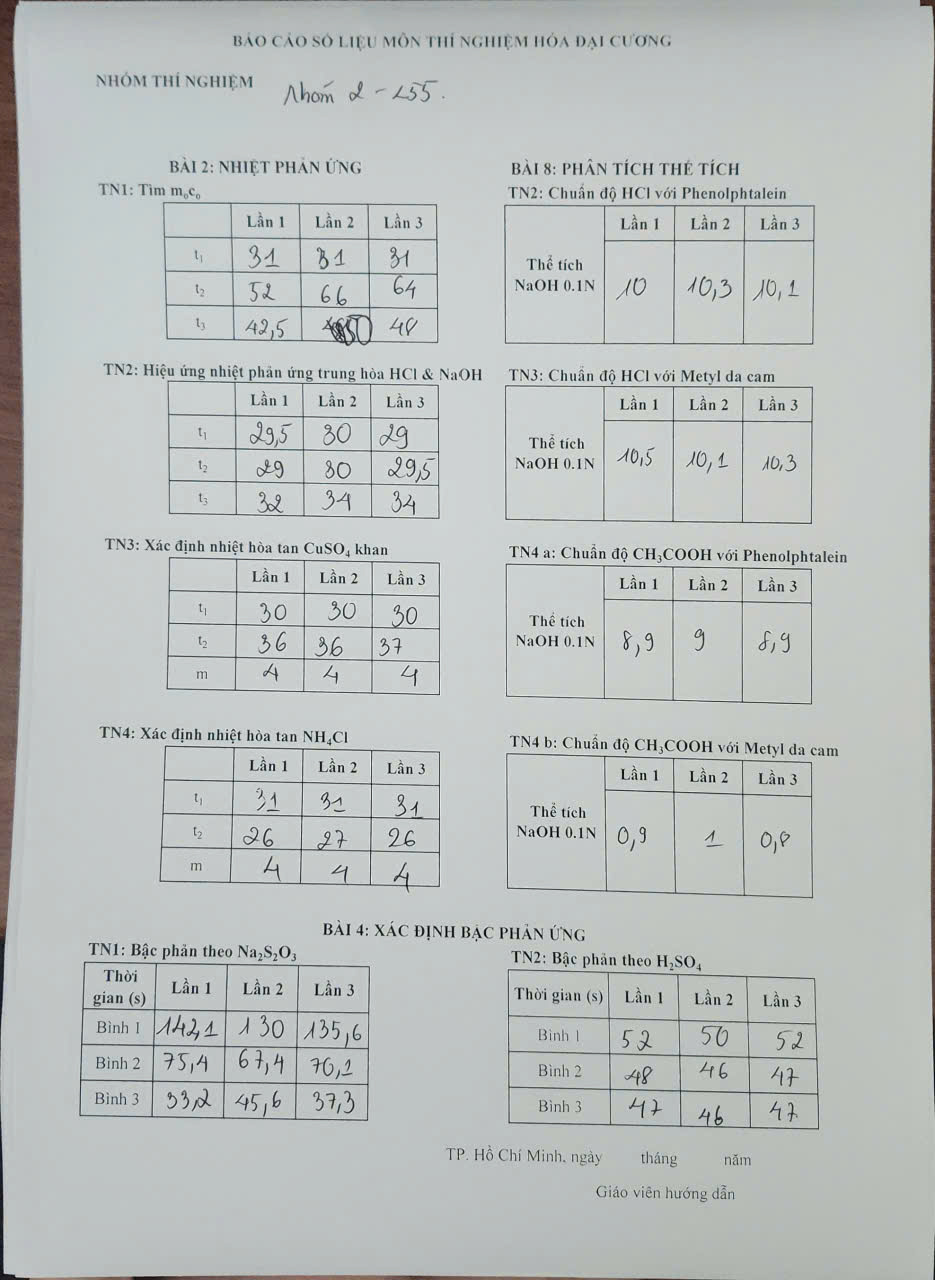
\includegraphics[max width=\linewidth, height=0.9\textheight, keepaspectratio]{baocaosolieuthinghiem.jpg}
    \caption{Bản báo cáo số liệu thực nghiệm gốc}
\end{figure}

%\bibliographystyle{plain}
%\bibliography{refs/example.bib}
%\nocite{*}

\end{document}
